\documentclass{article}

% --- load packages ---
\usepackage[margin=1in]{geometry} % change the margins
\usepackage{amsmath} % useful math environments and commands like align
\usepackage[colorlinks,bookmarks,bookmarksnumbered,allcolors=blue]{hyperref} % hyperlinks between references
\usepackage{graphicx}  % include images
\usepackage[table,xcdraw]{xcolor}
\usepackage[caption=false]{subfig} % subfigures.  false option prevents conflicts in caption styling with other packages
\usepackage{booktabs} % better tables
\usepackage[capitalise]{cleveref} % better referencing. uses cref.
\usepackage[section]{placeins} % sometimes useful to prevent figures from floating out of a section
\usepackage{cite} % handles multiple citations in one command better
\usepackage{doi} % allow correct hypderlinking of DOIs
\usepackage[normalem]{ulem}
\usepackage{float}
\usepackage{minted}
\usepackage{pdfpages}
\usepackage{tikz}
\usepackage{csvsimple}
\usepackage{adjustbox, lipsum}
\usepackage{setspace}
\usetikzlibrary{tikzmark}

\useunder{\uline}{\ul}{}
\newcommand{\wide}{0.7\linewidth}


\begin{document}
\singlespacing
\title{Unconstrained Optimization}
\author{Landon Wright}
% put in \date{} if you don't want a date to appear, or enter a specific date, otherwise default is today's date.
\maketitle
\section{Program Description}

\subsection{Steepest Descent}
The steepest descent method is the simplest of the optimization methods that are implemented here.  The search direction, $s$, is simply 
\begin{equation}
s = \nabla f(\textbf{x})
\end{equation}
Due to this the method is exceptionally simple to implement. It is however quite inefficient.  On both of the given equations it was the slowest to converge to the solution and required the highest number of function calls.  As a result it is an undesirable method.

\subsection{Conjugate Gradient}
The conjugate gradient method requires only a slight change to the steepest descent method for a large increase in efficiency.  The search direction is modified to become
\begin{equation}
s^{k+1} = - \nabla f^{k+1} + \beta^k s^k
\end{equation}

where
\begin{equation}
\beta^k = \frac{\left(\nabla f^{k+1}\right)^T \nabla f^{k+1}}{\left(\nabla f^{k}\right)^T \nabla f^{k}}
\end{equation}

This small change results in the method becoming one of conjugate directions which in turn makes the method significantly more powerful.  This is seen in the results of testing on the two given equations. The conjugate gradient method finds the optimum in fewer iterations and with less function calls.


\subsection{Quasi-Newton}
In testing done the Quasi-Newton method was shown to converge with the fewest number of iterations.  This is perhaps because it combines the far away efficiency of the steepest descent method with the power of conjugate gradient methods.  The result is a method the outperforms either of them on their own.  This power does come at the cost of additional complexity to implement.  The search direction is
\begin{equation}
s = -\textbf{N}\nabla f(\textbf{x})
\end{equation}
Which appears to be no more complicated than the other methods, however there is considerable complexity involved in determining \textbf{N} (For reference see equation 3.80 in the book).

\subsection{Step size}
The method of determining step size is the simple parabolic line search described in the book.  It is not the most efficient method, but it's simplicity is beneficial in ease of implementation.
\section{Testing Results}
\subsection{Function 1 Results}
% Steepest descent data
\begin{table}[H]
	\caption{Steepest descent progression}
	\centering
	\noindent\adjustbox{max width=\textwidth}{%
\begin{tabular}{|r|c|c|c|c|c|}
	\hline
  % \noindent\adjustbox{max width=\textwidth}{%
  & \bfseries Start-value & \bfseries Value & \bfseries Step-direction & \bfseries Step-len & \bfseries Function-calls
	%\\\hline
  \csvreader[head to column names]{output1.csv}{}%
  {\\\thecsvrow &(\a, \b, \c)& \d & (\e, \f, \g) & \h & \i}
  \\\hline
\end{tabular}}
\end{table}

% \csvautotabular{output1.csv}}

% Conjugate gradient data
% \noindent\adjustbox{max width=\textwidth}{%
% \csvautotabular{output2.csv}}
\begin{table}[H]
	\caption{Conjugate gradient progression}
	\centering
	\noindent\adjustbox{max width=\textwidth}{%
\begin{tabular}{|r|c|c|c|c|c|}
	\hline
  % \noindent\adjustbox{max width=\textwidth}{%
  &\bfseries Start-value & \bfseries Value & \bfseries Step-direction & \bfseries Step-len & \bfseries Function-calls

  \csvreader[head to column names]{output2.csv}{}%
  {\\\thecsvrow &(\a, \b, \c)& \d & (\e, \f, \g) & \h & \i}
  \\\hline
\end{tabular}}
\end{table}

% BFGS quasi-Newton data
% \noindent\adjustbox{max width=\textwidth}{%
% \csvautotabular{output3.csv}}
\begin{table}[H]
	\caption{Quasi-Newton progression}
	\centering
	\noindent\adjustbox{max width=\textwidth}{%
\begin{tabular}{|r|c|c|c|c|c|}
	\hline
  % \noindent\adjustbox{max width=\textwidth}{%
  &\bfseries Start-value & \bfseries Value & \bfseries Step-direction & \bfseries Step-len & \bfseries Function-calls

  \csvreader[head to column names]{output3.csv}{}%
  {\\\thecsvrow & (\a, \b, \c)& \d & (\e, \f, \g) & \h & \i}
  \\\hline
\end{tabular}}
\end{table}

\begin{table}[H]
	\centering
	\caption{Respective number of objective and gradient evaluations required to obtain minimum with tolerance of $1e^{-5}$ on the gradient}
	\label{my-label}
	\begin{tabular}{|l|r|r|}
		\hline
		\textbf{Method}    & \textbf{Objective Evaluations} & \textbf{Gradient Evaluations} \\
		Steepest descent   &                            254 &                            34 \\
		Conjugate Gradient &                             19 &                             4 \\
		Quasi-Newton       &                             19 &                             4 \\ \hline
	\end{tabular}
\end{table}

% table of obj evals and gradient evals for each method
\subsection{Rosenbrock Function Results}
% plot for steepest descent
\begin{figure}[H]
  \centering
  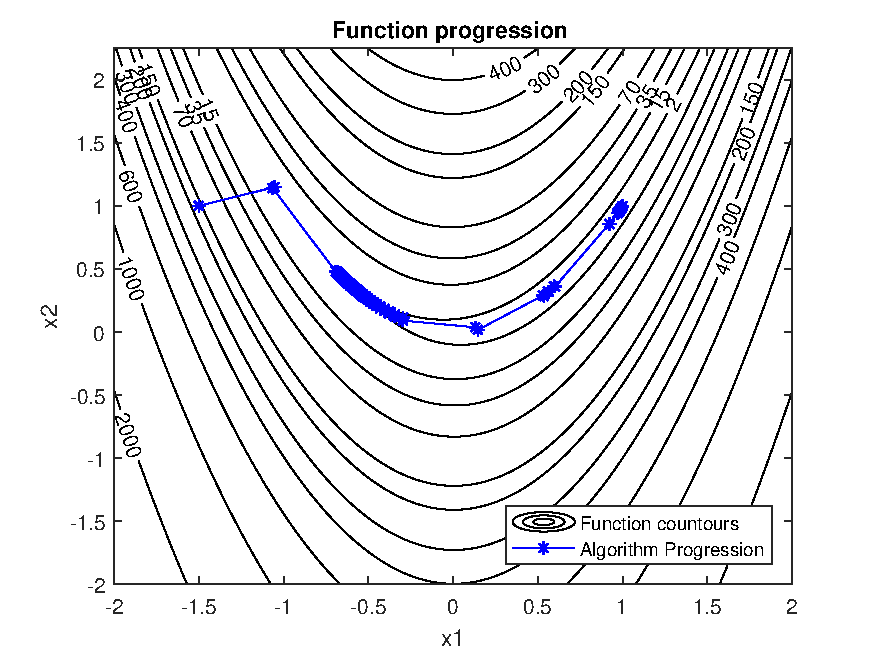
\includegraphics[width=\wide]{progression1.pdf}
  \caption{Progression of steepest descent algorithm}
  \label{fig:steepest1}
\end{figure}

% plot for conjugate gradient
\begin{figure}[H]
	\centering
	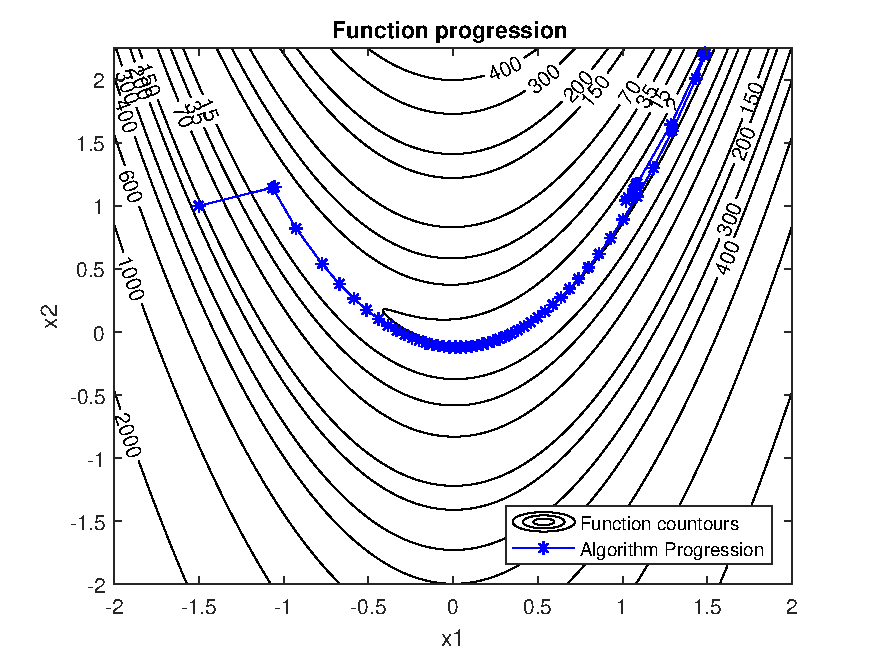
\includegraphics[width=\wide]{progression2.pdf}
	\caption{Progression of conjugate gradient algorithm}
	\label{fig:steepes2}
\end{figure}

% plot for quasi-Newton
\begin{figure}[H]
	\centering
	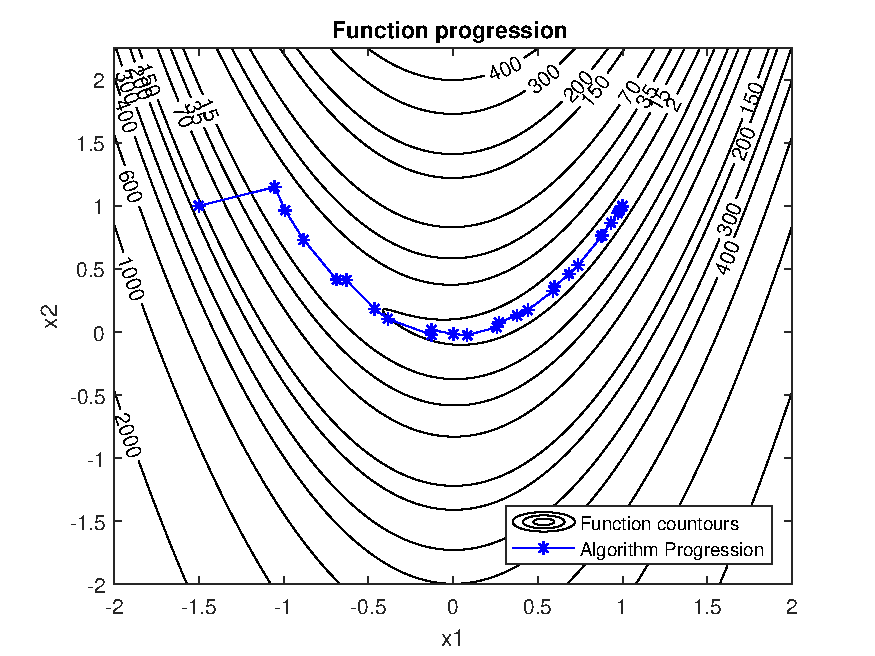
\includegraphics[width=\wide]{progression3.pdf}
	\caption{Progression of quasi-Newton algorithm}
	\label{fig:steepest3}
\end{figure}

\begin{table}[H]
	\centering
	\caption{Respective number of objective and gradient evaluations required to obtain minimum with tolerance of $1e^{-3}$ on the gradient}
	\label{my-label}
	\begin{tabular}{|l|r|r|}
		\hline
		\textbf{Method}    & \textbf{Objective Evaluations} & \textbf{Gradient Evaluations} \\
		Steepest descent   &                            931 &                           122 \\
		Conjugate Gradient &                            540 &                            77 \\
		Quasi-Newton       &                            172 &                            28 \\ \hline
	\end{tabular}
\end{table}
% table of obj and gradient evals for each method


\section{Matlab Code}

\subsection{Fminun Routine}
\inputminted[xleftmargin=10pt,linenos]{matlab}{fminun.m}
\subsection{Alpha* line search}
\inputminted[xleftmargin=10pt, linenos]{matlab}{aPrime.m}
\subsection{Driver}
\inputminted[xleftmargin=10pt,linenos]{matlab}{fminunDriv.m}

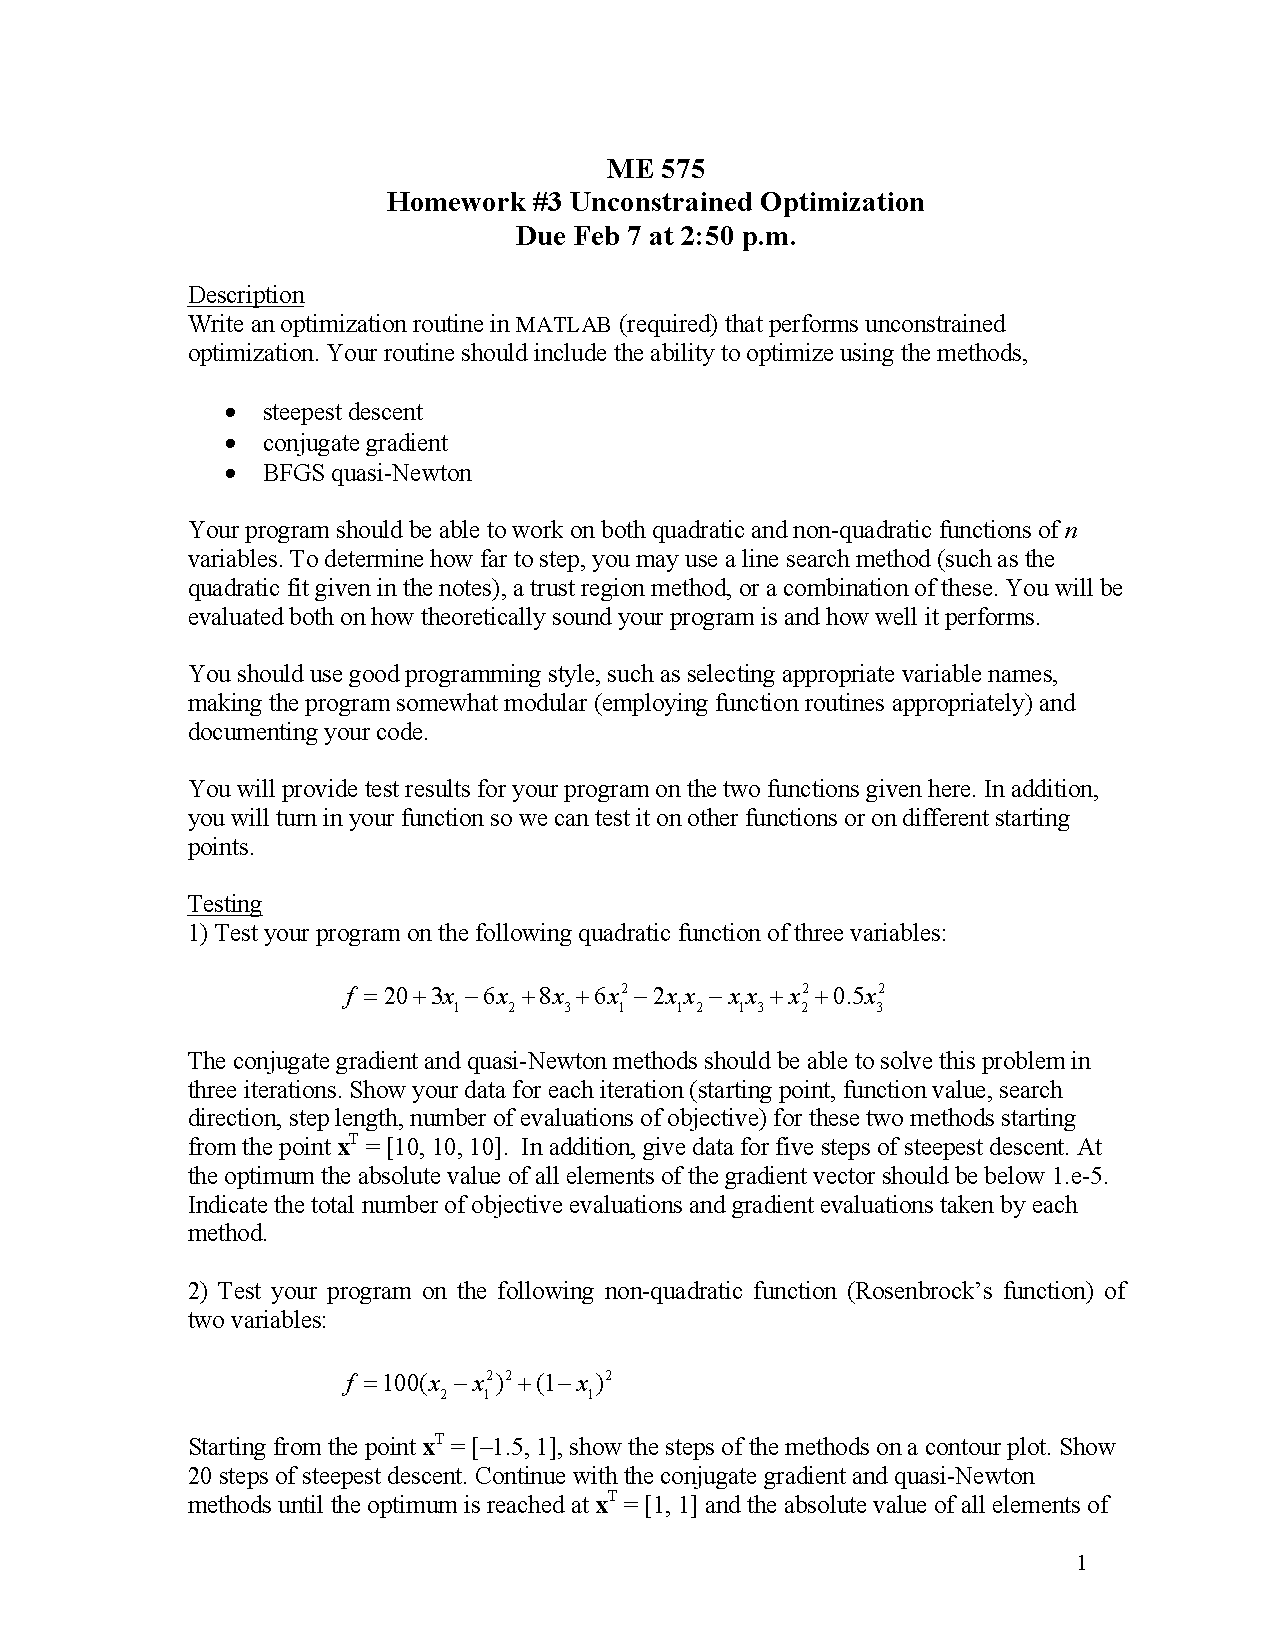
\includepdf[pages=-, pagecommand={}]{HW3Unconstrained.pdf}
\end{document}
